\hypertarget{rt__add_8c}{
\section{rt\_\-add.c File Reference}
\label{rt__add_8c}\index{rt_add.c@{rt\_\-add.c}}
}


\subsection{Detailed Description}
\begin{Desc}
\item[For internal use only.]
This file contains the implementation of the \hyperlink{group__dbprim__rbtree_ga7}{rt\_\-add()} function, used to add a red-black tree node to a given tree.\end{Desc}


Definition in file \hyperlink{rt__add_8c-source}{rt\_\-add.c}.

{\tt \#include \char`\"{}dbprim.h\char`\"{}}\par
{\tt \#include \char`\"{}dbprim\_\-int.h\char`\"{}}\par


Include dependency graph for rt\_\-add.c:\begin{figure}[H]
\begin{center}
\leavevmode
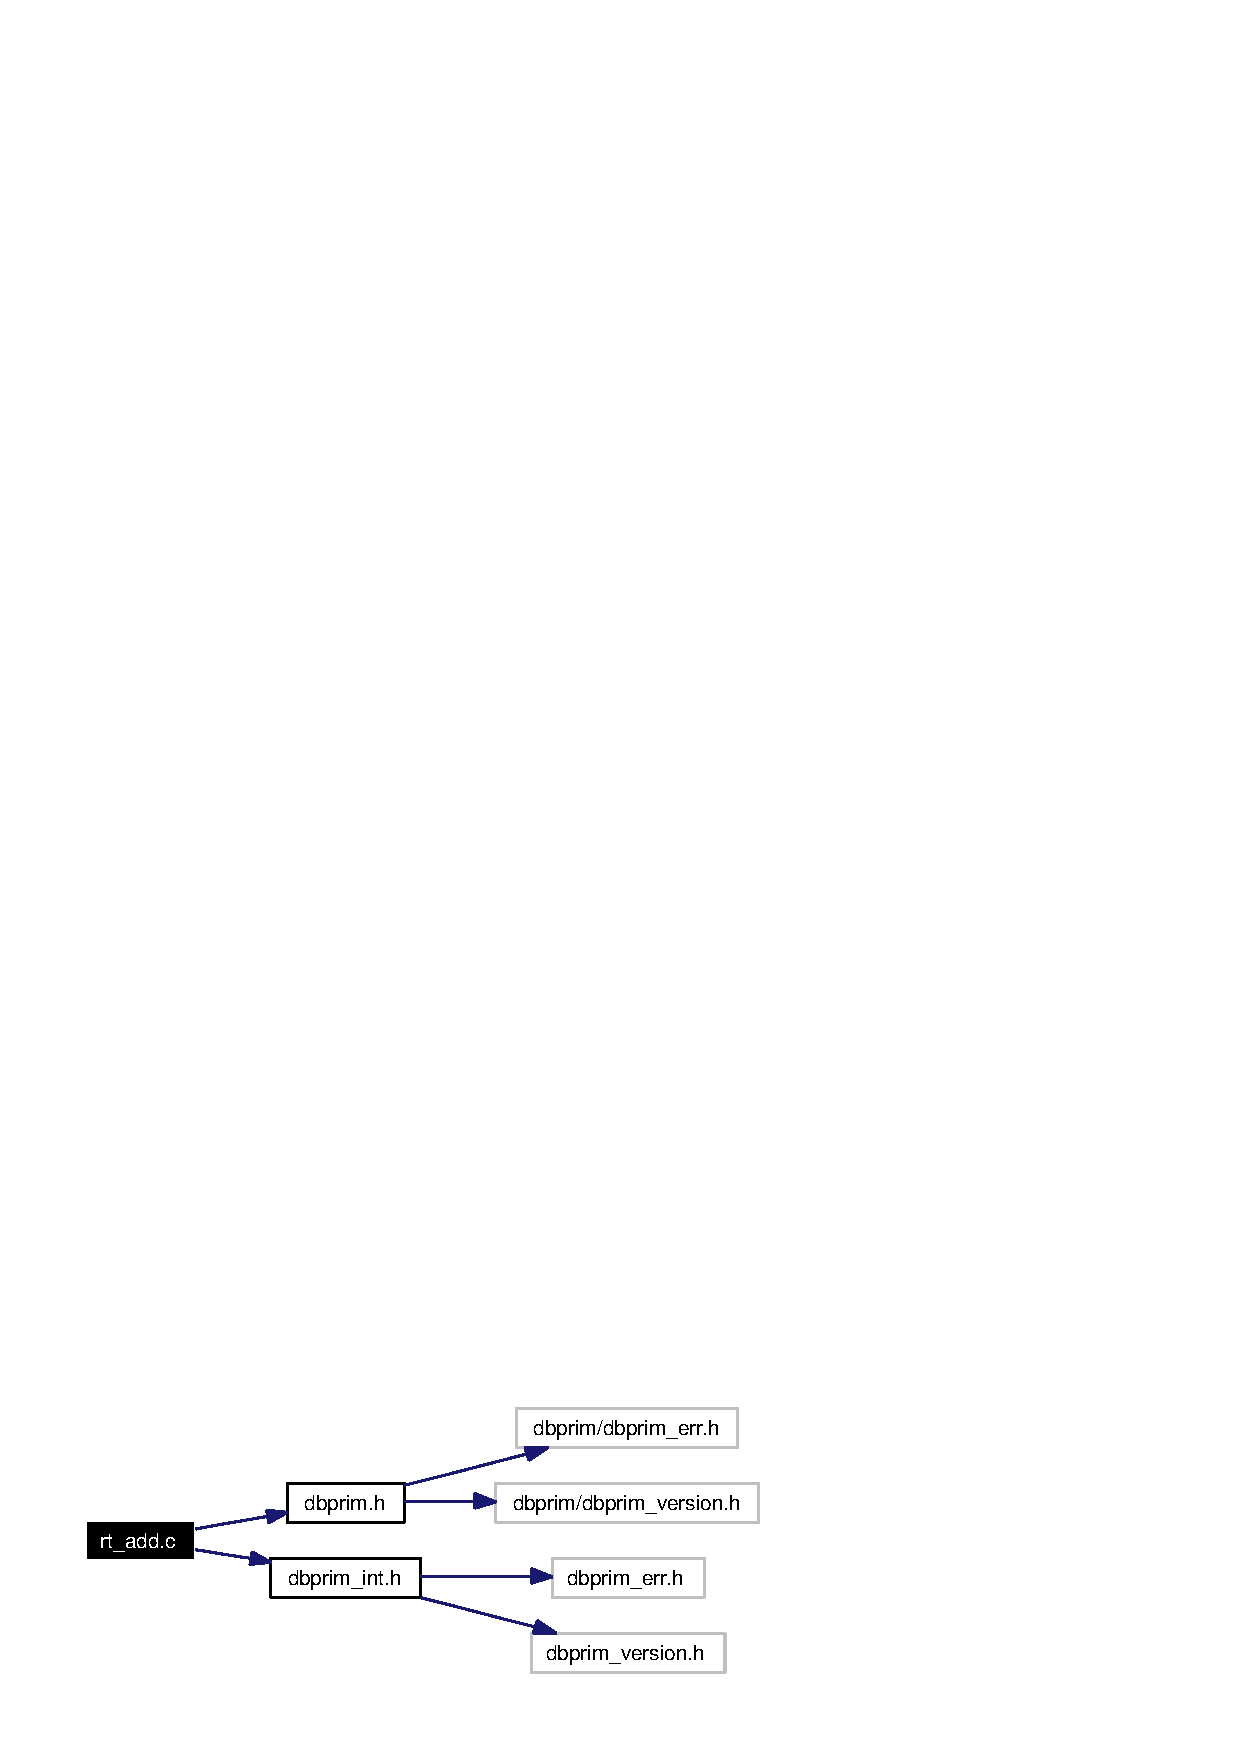
\includegraphics[width=184pt]{rt__add_8c__incl}
\end{center}
\end{figure}
\subsection*{Defines}
\begin{CompactItemize}
\item 
\#define \hyperlink{group__dbprim__rbtree_ga44}{uncle}(node)
\begin{CompactList}\small\item\em Locate the uncle of a node. \item\end{CompactList}\item 
\#define \hyperlink{group__dbprim__rbtree_ga45}{flip}(node)
\begin{CompactList}\small\item\em Flip the color of a node. \item\end{CompactList}\end{CompactItemize}
\subsection*{Functions}
\begin{CompactItemize}
\item 
unsigned long \hyperlink{group__dbprim__rbtree_ga7}{rt\_\-add} (\hyperlink{struct__rb__tree__s}{rb\_\-tree\_\-t} $\ast$tree, \hyperlink{struct__rb__node__s}{rb\_\-node\_\-t} $\ast$node, \hyperlink{struct__db__key__s}{db\_\-key\_\-t} $\ast$key)
\begin{CompactList}\small\item\em Add a node to a red-black tree. \item\end{CompactList}\end{CompactItemize}
